\documentclass{beamer}

\usepackage{tikz}
\usepackage{tikzducks,tikzlings}

\setbeamertemplate{background canvas}{
  \includegraphics[height=\paperheight]{Urquhart_Castle,_Loch_Ness,_Inverness,_Scotland_(17101840068)}
}
\setbeamertemplate{navigation symbols}{}

\begin{document}

\begin{frame}
  \begin{tikzpicture}[remember picture, overlay]
    \node[xscale=-1] at (2cm,-2.25cm) {
      \pgfmathparse{10*cos(\thepage)}
      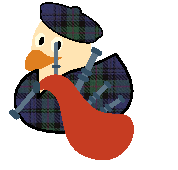
\includegraphics[angle=\pgfmathresult,origin=c,scale=0.75]{scot-duck-UF}
    };    
    \node at (4.5,-2.5) {
      \pgfmathparse{10*sin(\thepage)}	
      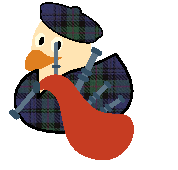
\includegraphics[angle=\pgfmathresult,origin=c,scale=0.8]{scot-duck-UF}
    };
    \node[xscale=-1] at (0.5cm,-3.5cm) {
      \pgfmathparse{10*sin(\thepage)}
      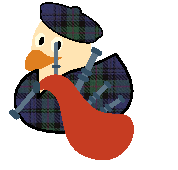
\includegraphics[angle=\pgfmathresult,origin=c]{scot-duck-UF}
    };
    \node at (7cm,-3.7cm) {
      \pgfmathparse{20*cos(\thepage)}
      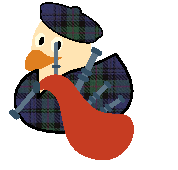
\includegraphics[angle=\pgfmathresult,origin=c,scale=1.05]{scot-duck-UF}
    };
    
    \node at ([yshift=0.2cm]current page.south) {\color{white}\Tiny Background image: \url{https://commons.wikimedia.org/wiki/File:Urquhart_Castle,_Loch_Ness,_Inverness,_Scotland_(17101840068).jpg}};
  \end{tikzpicture}
%	\pause[750]
\end{frame}	

\end{document}